\documentclass[border=5pt, tikz,convert={outfile=\jobname.png}]{standalone}
\usepackage{newtxtext}
\usepackage{xcolor}
%\usetikzlibrary{...}% tikz package already loaded by 'tikz' option
% \tikzset{curveinscope/.style={every path/.style={draw=black, text=black}}}
% \pagecolor[rgb]{0.8,0.8,0.8}
\begin{document}
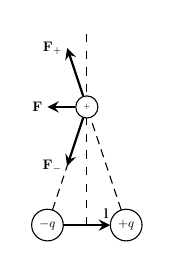
\begin{tikzpicture}[scale=0.5, every node/.style={scale=0.5}]
  \node[draw=black,fill=white, circle] (A) at (-1, 0) {\small $-q$};
  \node[draw=black,fill=white, circle] (B) at (1, 0) {\small $+q$};
  \draw[->,>=stealth, thick] (A) -- node[above=0.3cm, right=0.3cm] {$\mathbf{l}$} (B);
  \draw[dashed] (0,0) -- (0,5);
  \node[draw=black,fill=white, circle] (Q) at (0,3) {\tiny $+$};
  \draw[densely dashed] (A) -- (Q);
  \draw[->,>=stealth, thick] (Q) -- ++(-0.5, -1.5) node[left] {$\mathbf{F}_{-}$};
  \draw[densely dashed] (B) -- (Q);
  \draw[->,>=stealth, thick] (Q) -- ++(-0.5, 1.5) node[left] {$\mathbf{F}_{+}$};
  \draw[->,>=stealth, thick] (Q) -- ++(-1, 0) node[left] {$\mathbf{F}$};
\end{tikzpicture}
\end{document}